\chapter{Background} \label{chap:background}

This chapter will discuss the theoretical background needed to understand the protocol presented in this thesis. We will cover the main network protocols used in distributed systems, such as Request-Response and Publish-Subscribe, and how they can be applied to IoT devices. We will also discuss Universal Location Referencing, Space-Filling Curves, and Privacy-Preserving techniques, such as Homomorphic Encryption, which are the foundation of the solution proposed.

\section{Request-Response Protocol}

Request-response is a fundamental communication pattern in distributed systems where a client sends a request to a server and waits for a response. This synchronous communication model is characterized by its simplicity and direct interaction between parties, making it suitable for operations requiring immediate feedback and confirmation.

\subsection{HTTP}
HTTP (Hypertext Transfer Protocol) is the foundation of data communication on the World Wide Web. It operates as a request-response protocol, allowing clients to request resources from servers and receive responses. HTTP supports various methods (GET, POST, PUT, DELETE) for different types of operations and is extensible through headers and status codes.

\subsubsection{HTTPS}
HTTPS is a version of HTTP built on the SSL/TLS protocol, providing secure communication over a computer network. It encrypts data exchanged between clients and servers, ensuring confidentiality and integrity. HTTPS is essential for protecting sensitive information from eavesdropping and tampering.

One of the key features of HTTPS is its use of certificates to authenticate the server, ensuring that clients are communicating with the intended entity. This is possible through a relatively high usage of computational resources, which is a trade-off for the enhanced security it provides.

\subsection{Request-Response in IoT devices}
HTTPS is a commonly used choice also for IoT devices. However, its usability is often limited due to several factors:
\begin{itemize}
    \item \textbf{Resource Constraints\cite{mazhar2023iotsecurity}}: Encrypting and decrypting certificate standards (RSA, EEC, AES) can be computationally expensive, which is a significant concern for IoT devices with limited processing power and memory.
    \item \textbf{Lack of Secure Firmware Updates\cite{cyberark2024iot}}: Many IoT devices do not support secure firmware updates, making it difficult to patch vulnerabilities in the HTTPS implementation.
    \item \textbf{Weak or Nonexistent Certificate Validation\cite{bishopfox2020weakcertificates}}: Many IoT devices do not validate server certificates properly, leading to potential vulnerabilities.
\end{itemize}

This limitation has led to the development of alternative protocols and standards that are more suitable for IoT devices, such as CoAP (see \cref{sec:coap}) and MQTT (see \cref{sec:mqtt}). These protocols are designed to be lightweight and efficient, making them more suitable for resource-constrained devices.

\subsection{CoAP} \label{sec:coap}

CoAP (Constrained Application Protocol) is a specialized web transfer protocol designed for constrained devices and low-power networks\cite{rfc7252}. It operates over UDP, making it lightweight and suitable for IoT applications. CoAP supports request-response interactions similar to HTTP but is optimized for low-bandwidth and high-latency environments.

The protocol presents several key features:
\begin{itemize}
    \item Web protocol fulfilling M2M requirements in constrained
      environments.
    \item UDP-based with support for multicast.
    \item Low header overhead and parsing complexity.
    \item URI and Content-type support.
    \item Simple proxy and caching capabilities.
    \item A stateless HTTP mapping, allowing proxies to be built providing access to CoAP resources via HTTP in a uniform way or for HTTP simple interfaces to be realized alternatively over CoAP.
    \item Security binding to Datagram Transport Layer Security (DTLS)
\end{itemize}

Due to its design, CoAP can replicate the RESTful architecture of HTTP, supporting methods such as GET, POST, PUT, and DELETE. Additionally, CoAP provides an \textit{observe} mechanism that enables clients to subscribe to resources and receive notifications upon changes.

Henceforth, references to HTTP requests could be interpreted as referring to a \textbf{CoAP request}. Moreover, my protocol is designed to be compatible with IoT devices where bandwidth, data rate, and power consumption are critical factors. CoAP's lightweight nature and efficient use of resources make it a suitable choice for such applications.

\section{Publish-Subscribe Protocol}
Publish-Subscribe (Pub/Sub) is an asynchronous messaging pattern where senders (publishers) categorize messages into topics without the knowledge of the receivers (subscribers). Subscribers express interest in specific topics and receive messages published on those topics. This decoupled architecture enables scalable and flexible communication in distributed systems.

\subsection{MQTT} \label{sec:mqtt}
MQTT (Message Queuing Telemetry Transport) is a lightweight, open-source messaging protocol designed for constrained devices and low-bandwidth, high-latency networks. It implements the publish-subscribe pattern over TCP/IP, providing three quality service levels for message delivery and supporting various security features.

The protocol defines three main network entities:
\begin{itemize}
    \item \textbf{Message Broker}: The central component that manages message routing between publishers and subscribers. It receives messages from publishers and forwards them to subscribers based on their subscriptions.
    \item \textbf{Publisher}: A client that sends messages to the broker on specific topics. 
    \item \textbf{Subscriber}: A client that expresses interest in specific topics and receives messages published to those topics by the broker.
\end{itemize}

\subsubsection{MQTT Quality of Service Levels}

MQTT provides three quality of service (QoS) levels to ensure message delivery reliability:
\begin{itemize}
    \item \textbf{QoS 0 (At most once)}: The message is delivered at most once, with no acknowledgment from the receiver. This level is suitable for applications where occasional message loss is acceptable.
    \item \textbf{QoS 1 (At least once)}: The message is guaranteed to be delivered at least once, with acknowledgment from the receiver. This level ensures that messages are not lost but may result in duplicates.
    \item \textbf{QoS 2 (Exactly once)}: The message is guaranteed to be delivered exactly once, using a four-step handshake process. This level provides the highest reliability but incurs more overhead.
\end{itemize}

\subsubsection{MQTT Security}

As we mentioned, one of the key features of MQTT is the possibility to scale the protocol to fit the needs of the application. This is possible by using different security features, such as TLS/SSL for secure communication, authentication mechanisms to verify client identities, and access control lists to restrict topic access. These features help protect against unauthorized access and ensure the integrity of messages exchanged between clients.

\subsubsection{MQTT Workflow}

\begin{figure}[h]
    \centering
    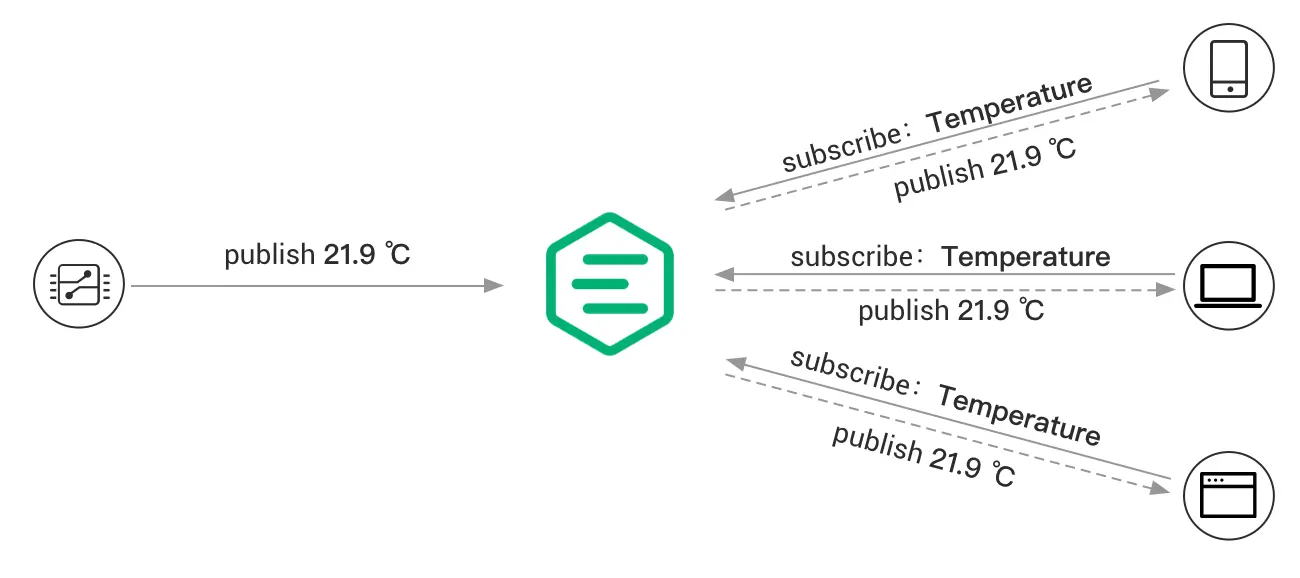
\includegraphics[width=\columnwidth]{img/mqtt-workflow-example.png}
    \caption{MQTT Workflow}
    \label{fig:mqtt-workflow}
\end{figure}

Generally, the MQTT workflow starts with the client establishing a connection to the broker, using a TCP/IP connection with optional TLS/SSL security. Once connected, the client can publish messages to specific topics or subscribe to topics of interest. The broker then routes messages to subscribers based on their subscriptions (see \cref{fig:mqtt-workflow}).

\subsection{LA-MQTT} \label{sec:la-mqtt}
LA-MQTT~\cite{montori2022lamqtt} extends the standard MQTT protocol by incorporating location-based features. It enables spatial queries and location-aware message routing, making it particularly suitable for IoT applications requiring geographical context in message distribution.

The protocol is first introduced to resolve the limitations of traditional MQTT in handling location-based data.

\begin{table}[h]
\small
\begin{tabularx}{\linewidth}{|l|X|X|X|p{4cm}|}
\hline
\textbf{API} & \textbf{Subject} & \textbf{MQTT OP} & \textbf{Topic} & \textbf{Payload} \\ \hline
Position publish & MC & Publish & GPS\_DATA & $\{position: ( P_i )\}$ \\ \hline
Topic subscription & MC & Subscribe & $C(i, t_s)$ & * \\ \cline{2-5}
 & MC & Publish & MC\_SUB & $\{ mc: i, topic: t_s \}$ \\ \hline
Geo fence publish & LDS & Publish & GEO\_FENCE\_DATA & $\{topic: t_s, content: c_s, $\newline$region: g_s, event: e_s\}$ \\ \hline
Content publish & Backend & Publish & $C(i, t_s)$ & $\{content: c_s\}$ \\ \hline
\end{tabularx}
\caption{The LA-MQTT Publish-subscribe Operations}
\label{table:la-mqtt}
\end{table}

Table \ref{table:la-mqtt} summarizes the main operations of the LA-MQTT protocol, highlighting the interactions between clients (MC), location data sources (LDS), and the backend system.

Those operations include:
\begin{itemize}
    \item \textbf{Position Publish}: MC publishes their GPS data to the broker, allowing other clients to receive updates on their positions.
    \item \textbf{Topic Subscription}: MCs subscribe to specific topics, enabling them to receive messages related to their areas of interest.
    \item \textbf{Geo fence Publish}: LDSs publish geo fence data, which includes the topic, content, region, and event associated with the Geo fence.
    \item \textbf{Content Publish}: The backend publishes content related to the subscribed topics, forwarding it to the subscribed MCs.
\end{itemize}

LA-MQTT integrates two privacy-preserving strategies within its client-side architecture:
The first strategy is based on randomized location perturbation. This method applies controlled noise to the GPS coordinates before transmission. Specifically, for a given GPS value $P_i$, a user-defined number of decimal digits is preserved, while the remaining digits are randomly replaced. This approach balances between:
\begin{itemize}
    \item Privacy Preservation (PP): Higher randomness enhances anonymity.
    \item Spatial Precision (SP): Excessive perturbation can degrade the accuracy of spatial notifications.
\end{itemize}
The second strategy involves the use of dummy updates. Here, the MC alternates between sending real and synthetic (dummy) location data. In each sequence of updates, only one is the actual position; the others are randomly generated or trajectory-based decoys.

\section{Universal Location Referencing}
Universal Location Referencing provides standardized methods for encoding and representing geographical locations. These systems ensure consistent and unambiguous location representation across different applications and platforms.

\subsection{Background: Distance Measures Between Vectors}
\label{sec:background-distances}

In many applications, especially related to positioning and spatial data, it is essential to measure the similarity or dissimilarity between vectors. This is particularly relevant in fields such as machine learning, computer vision, and geographic information systems. To analyze similarity or dissimilarity between vectors $\mathbf{x}, \mathbf{y} \in \mathbb{R}^n$, three standard distance metrics are:

\begin{description}
  \item[Cosine similarity:]
  \[
    \mathrm{CS}(\mathbf{x}, \mathbf{y}) 
    = \frac{\sum_i x_i y_i}{\|\mathbf{x}\| \cdot \|\mathbf{y}\|}.
  \]
  This measures the angle between vectors and is scale‑invariant.

  \item[Euclidean distance:]
  \[
    \mathrm{ED}(\mathbf{x}, \mathbf{y}) 
    = \sqrt{\sum_i (x_i - y_i)^2}.
  \]
  It represents the straight-line distance but involves a non-linear square root.

  \item[Manhattan distance:]
  \[
    \mathrm{MD}(\mathbf{x}, \mathbf{y}) 
    = \sum_i |x_i - y_i|.
  \]
  Also known as the $\ell_1$ norm, it sums up absolute differences.
\end{description}
\subsection{Cantor Pairing}

Cantor Pairing is a mathematical technique that uniquely maps two natural numbers to a single natural number (\cref{fig:cantor}). This bijective function $\pi: \mathbb{N} \to \mathbb{N}$ is particularly useful in computer science for combining two coordinates into a single value while maintaining the ability to recover the original coordinates.

More formally, the Cantor pairing function is defined as:
\[
    \pi(x, y) = \frac{(x + y)(x + y + 1)}{2} + y
\]

Although this function does not preserve algebraic properties, it provides some unique properties derived from the fact that it segments the two-dimensional space into a zig-zag pattern.

\[
    \pi(x, y) + 1 = \pi(x - 1, y + 1)
\]

Moreover, we also need to define the behavior of the function when one hits the boundaries of the first quadrant:

\[
    \pi(x, 0) + 1 = \pi(x + 1, 0)
\]

At last, we denote the starting point of the Cantor pairing function as \( \pi(0, 0) = 0 \). This means that the function starts at the origin of the two-dimensional space and maps it to zero in the one-dimensional space. The inverse of the Cantor pairing function can be computed as follows:
\[
    \pi^{-1}(z) = \left( \frac{n(n + 1)}{2} - z, z - \frac{n(n + 1)}{2} \right)
\]
Where \( n \) is the largest integer such that \( \frac{n(n + 1)}{2} \leq z \). This allows us to retrieve the original coordinates \( (x, y) \) from the single value \( z \).

This function is widely used in computer science, particularly in data structures and algorithms, where it is necessary to map multi-dimensional data to a single dimension for efficient storage and retrieval. It is also used in various applications such as database indexing, spatial data representation, and cryptography.


\vspace{5mm}

\begin{figure}[h]
    \centering
    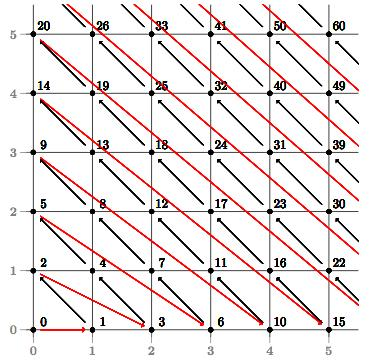
\includegraphics[width=6.5cm,height=4.7cm]{img/cantor-pairing.jpg}
    \caption{Visualization of the Cantor pairing function mapping two-dimensional coordinates to a single value}
    \label{fig:cantor}
\end{figure}

\vspace{5mm}

\section{Space Filling Curves}
Space-filling curves are mathematical curves that pass through every point in a multi-dimensional space. They provide a way to map multi-dimensional data to a single dimension while preserving spatial locality, making them valuable for spatial indexing and data organization.

The most common space-filling curves include (\cref{fig:space-filling}):
\begin{itemize}
    \item \textbf{Z-order Curve}
    \item \textbf{Hilbert Curve}
\end{itemize}

%\vspace{5mm}

\begin{figure}[h]
    \centering
    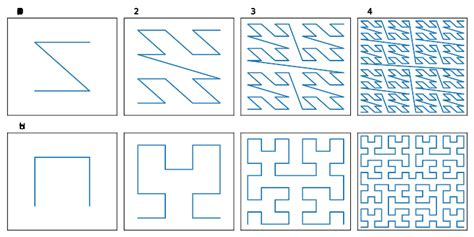
\includegraphics[width=6.5cm,height=4.7cm]{img/hilbert-z-order.jpg}
    \caption{Comparison of Z-order and Hilbert curves in two-dimensional space}
    \label{fig:space-filling}
\end{figure}

\vspace{5mm}

The Hilbert Curve is particularly notable for its ability to preserve locality, meaning that points that are close in multi-dimensional space remain close in the one-dimensional representation.

On the other hand, the Z-order Curve, preserves the order of positions in a grid-like manner, making it suitable for applications requiring efficient spatial queries. Thus, it's possible to reduce the problem of finding matching points to finding the maximum prefix of two-bit strings.

\subsection{Z-order Curve} \label{sec:z-order-curve}
As mentioned, the Z-order curve is one of the most widely used space-filling curves. It maps multi-dimensional data into a single dimension, similar to the Cantor encoding function. Conversely, it has some useful properties, when applied to spatial data, such as preserving locality and allowing efficient range queries.

\subsubsection{Z-order Encoding}

The encoding process for Z-order involves interleaving the bits of the coordinates of a point in a multi-dimensional space. For example, given a point with coordinates \( (x, y) \), the Z-order encoding can be represented as:
\[
    Z(x, y) = \sum_{i=0}^{n} (x_i \cdot 2^{2i} + y_i \cdot 2^{2i+1})
\]

Where:
\begin{itemize}
    \item \( x_i \) and \( y_i \) are the bits of the binary representation of the coordinates \( x \) and \( y \).
    \item \( n \) is the number of bits used to represent each coordinate.
\end{itemize}

The Z-order curve can also be applied to encode vectors with dimensions greater than two. In this case, the encoding process involves interleaving the bits of all coordinates in a similar manner.


\subsubsection{Z-order Decoding}
The decoding process retrieves the original coordinates from the Z-order encoded value. Given a Z-order value \( Z \), the decoding can be performed by extracting the bits corresponding to each coordinate:
\[
    x = \sum_{i=0}^{n} (Z \pmod{ 2^{2i+2} }) \cdot 2^i
\]
Where:
\begin{itemize}
    \item \( Z \pmod{ 2^{2i+2} } \) extracts the bits corresponding to the \( i \)-th coordinate.
    \item The result is then shifted and combined to reconstruct the original coordinate \( x \).
\end{itemize}

The same process can be used to find the $y$ value by de-interleaving the other bits.

\subsubsection{Z-order Querying}
Let us consider a scenario where we want to find all points within a specific range in a two-dimensional space. We define \( P \) as the set of points in the space, and we want to find all points \( p \in P \) such that:
\[
    p.x \in [x_{min}, x_{max}] \quad \text{and} \quad p.y \in [y_{min}, y_{max}]
\]

We can leverage the Z-order encoding to efficiently query this range. This is possible by calculating the order of the encoding that we want to find. 
By definition, we can represent the GPS coordinates of a point \( (x_p, y_p) \) into a point \( e_p \). This point will be represented in the space of \( n \) orders, each contained in \( \mathbb{Z}_4 \).

\subsubsection{Maximum Common Prefix Search}
A key operation in Z-order-based spatial queries is finding the maximum common prefix between two Z-order encoded values. This operation is fundamental for determining spatial relationships between points.

Given two Z-order encoded values \( Z_1 \) and \( Z_2 \), we can find the maximum common prefix by following three steps. Firstly, we convert both values to their binary representation. Then, we compare the bits from left to right, stopping at the first position where the bits differ. Finally, we extract the common prefix up to that point. The cited algorithm shows that in the worst case, the maximum common prefix can be found in \( O(n) \) time, where \( n \) is the number of bits in the Z-order encoding.

The length of the common prefix determines the size of the smallest bounding box that contains both points. This property is particularly useful for:
\begin{itemize}
    \item Finding the smallest region containing multiple points
    \item Determining if points are within a certain distance of each other
    \item Optimizing spatial range queries
\end{itemize}

For example, consider two points with Z-order encodings:
\begin{align*}
    Z_1 &= 3310_4 \\
    Z_2 &= 3312_4
\end{align*}
The maximum common prefix is \( 331_4 \), indicating that these points share the same region in the first three orders of the encoded space. We used base 4 because it's the easiest way to visualize which of the four quadrants the point belongs to, as each digit represents a quadrant in a two-dimensional space.

This prefix-based approach can be extended to handle a range of queries by:
\begin{enumerate}
    \item Encoding the query range boundaries
    \item Finding the maximum common prefix of the range
    \item Generating all possible Z-order values that share this prefix
\end{enumerate}

The efficiency of this approach comes from the fact that we can perform these operations using simple bitwise operations, making it suitable for real-time applications.


\section{Privacy Preserving Techniques}
Privacy-preserving techniques ensure the protection of sensitive information while allowing necessary computations and data processing. These methods are crucial in maintaining confidentiality in distributed systems and data analysis. For example, in the context of location-based services, privacy-preserving techniques allow for the sharing of location data without revealing exact coordinates, thus protecting user privacy.

\subsection{Homomorphic Encryption}
Homomorphic Encryption(HE) is a form of encryption that allows specific types of computations to be performed on cipher text, producing an encrypted result that, when decrypted, matches the result of operations performed on the plain text.

Let us denote \( \xi_k \) the encryption function, \( \xi_k^{-1} \) the decryption function, and \( f \) a function that can be computed on plain texts. Homomorphic Encryption satisfies the property:

\[
    \xi_k(f(x)) = f(\xi_k(x))
\]

In recent years, several Homomorphic Encryption schemes have been proposed, each with different properties and capabilities. The scheme used in this thesis is the Brakerski-Gentry-Vaikuntanathan (BGV, 2011) scheme \cite{Brakerski2012-wj}, which is a leveled fully homomorphic encryption scheme that supports both addition and multiplication operations on encrypted data. The BGV scheme is particularly notable for its efficiency and ability to handle large integers, making it suitable for practical applications in privacy-preserving computations.
This scheme was based on the security of \textbf{(Ring) Learning With Errors} (RLWE) (see \cref{sec:rlwe}) problem, which is a hard problem in lattice-based cryptography. The need for such a scheme arises from the increasing demand for secure computations in various fields, including cloud computing, data analysis, and machine learning. This type of new technology is designed to resist quantum computers and cryptanalysis. 

\subsubsection{Security foundation: (Ring) Learning With Errors (RLWE)} \label{sec:rlwe}

The security of lattice-based FHE schemes, especially BGV, rests on the hardness of the Ring Learning With Errors (RLWE) problem, a ring-based variant of the Learning With Errors (LWE) problem introduced by Lyubashevsky, Peikert, and Regev in 2010 \cite{Lyubashevsky2010-jo}.
In RLWE, one works over a polynomial ring modulo both a prime $q$ and an irreducible polynomial $a(x)$:

\[
    a(x) = a_0 + a_1 x + \ldots + a_{n-1} x^{n-1}, \text{where } a_i \in \mathbb{Z}_q
\]

Samples are of the form $(a(x),\,b(x)=a(x)s(x)+e(x))$, where $e(x)$ is a small “error” polynomial. Recovering $s(x)$ given many such samples is presumed hard, based on reductions to the Shortest Vector Problem (SVP) in ideal lattices.

\subsection{Homomorphic Encryption Types}

\textbf{Fully Homomorphic Encryption (FHE)} allows the evaluation of arbitrary circuits of additions and multiplications over encrypted data, without decryption. However, earlier FHE schemes suffered from inefficiencies, particularly due to the large growth of noise. The BGV scheme answered these challenges by avoiding Gentry’s “bootstrapping” \cite{Brakerski2012-wj} step via \emph{leveled} evaluation, and controlling noise through \emph{modulus switching} and \emph{relinearization} techniques.

\textbf{Partially Homomorphic Encryption (PHE)} supports only one type of operation—either addition (e.g., Paillier) or multiplication (e.g., RSA variants). These are faster than FHE but limited in expressiveness, making them suitable for simpler tasks where only one operation type is required.

\subsection{HE Translation Key} \label{sec:translation-key}

Originally introduced in 1998, Blaze, Bleumer, and Strauss (BBS)\cite{Blaze1998-cw} proposed an application called atomic proxy re-encryption, the mechanism enables ciphertexts encrypted under one public key to be transformed into ciphertexts decryptable under another key—without exposing the underlying plaintexts or private keys. It addresses the challenge of heterogeneity in multi‑actor systems, eliminating the need for a central trusted broker to perform decryption and re‑encryption. Instead, each data owner can generate a *Translation Key* that authorizes on‑the‑fly ciphertext conversion by other parties.

Consider a privacy‑preserving workflow involving three participants—Alice, Bob, and Charlie—each with their respective keypairs $(k_A^+, k_A^-)$, $(k_B^+, k_B^-)$, and $(k_C^+, k_C^-)$. Suppose Alice wants to store encrypted data on Bob’s untrusted server. She encrypts her data under $k_A^+$ and uploads the ciphertext. Since Bob cannot decrypt (he lacks $k_A^-$), Charlie would also be unable to access the data directly. However, if Alice generates and distributes a Translation Key $k_{A\to C}$, Charlie can convert the ciphertext into one encrypted under $k_C^+$ and then decrypt it with $k_C^-$, without learning Alice’s private key or Bob’s data.

The Translation Key creation requires Alice's Private key and Charlie's Public key, ensuring that only authorized parties can perform the conversion.

\[
    k_{A\to C} = f(k_A^-,k_C^+)
\]

By allowing secure key-conditional ciphertext conversion, the Translation Key mechanism preserves confidentiality across distinct encryption domains. This is particularly valuable when multiple data owners—with different keys—need to perform joint encrypted computations on a shared ciphertext under a common key.


\section{Usage of HE for Matching}
Homomorphic Encryption can be used to securely match location. To archive this, we can use different techniques such as:
\begin{itemize}
    \item \textbf{Distance Calculation}: It is archived by tweaking the distance calculation algorithms (mentioned before in \cref{sec:background-distances} e.g., Euclidean distance, Cosine similarity, Manhattan Distance) to work with encrypted coordinates. The main limit comes with the constraint that the operations must be compatible with the encryption scheme used. For instance, calculating the square Euclidean distance between two points \( (x_1, y_1) \) and \( (x_2, y_2) \) can be expressed as:
    \[
        d^2 = (x_1 - x_2)^2 + (y_1 - y_2)^2
    \]
    That can be computed homomorphically and then decrypted before computing the square root to get the actual distance. We will further discuss this in the Testing Section \ref{sec:testing-performance}.
    \item \textbf{Encoding Coordinates}: By encoding coordinates into a grid-like structure, we can reduce the problem into finding two different points sharing the same area-encoding. This approach comes with some limitations, mainly related to the precision of the approximation and the size of the grid. Still, it allows for efficient matching of points within a specific area without revealing their exact coordinates. This is done by applying a space-filling curve, such as Z-order (\cref{sec:z-order-curve}), to the coordinates.
\end{itemize}

\subsubsection{Privacy-Preserving Z-order Queries} \label{sec:privacy-preserving-z-order}

When implementing privacy-preserving location queries using Z-order encoding, we can employ homomorphic encryption to protect sensitive location data \cite{zhang2020privacy}. Let us consider a scenario where a user \( A \) wants to share their location with user \( B \) while maintaining privacy:

\begin{itemize}
    \item Let \( QK_A \) be the QuadKey representation of \( A \)'s location
    \item Let \( M_B \) be the bit mask specified by \( A \) for user \( B \)
    \item The service provider (SP) performs homomorphic multiplication: \( QK_A \otimes M_B \)
\end{itemize}

To ensure unambiguous results, we increment each value in \( qk_i \in QK_A \) by one before encryption, such that \( qk_i \in \{1,2,3,4\} \). In this scheme \cite{zhang2020privacy}:
\begin{itemize}
    \item A bitmask value of 1 preserves the location data
    \item A bitmask value of 0 masks the location data
\end{itemize}

After decryption on the client device, we:
\begin{enumerate}
    \item Remove any zero values
    \item Convert the elements back to \( \mathbb{Z}_4 \)
    \item Generate a masked QuadKey string that produces a bounding box with the desired level of detail
\end{enumerate}

This approach is computationally efficient as it requires only one round of homomorphic multiplication. The resulting bounding box effectively hides both precise locations and movement patterns, providing privacy even against colluding users.

For example, given a precise GPS coordinate \( (43.084451, -77.680069) \), the system can generate bounding boxes of varying sizes based on the privacy preferences (where the distance \( d \) represents the level of detail). This ensures that location data is shared at an appropriate granularity while maintaining user privacy.

% TODO: add other type of queries

\subsection{PHE and FHE Implications}

The choice between Partially and Fully Homomorphic Encryption has significant implications for system performance, security, and functionality. As previously discussed, the two methods used for proximity checks in a location-based scenario require careful consideration of the encryption scheme.

If the requirements only involve checking whether two positions share a common area, leveraging the speed and simplicity of the Z-order approach is recommended. This method allows the usage of PHE to perform fast proximity checks without significant overhead. As we have seen in \cref{sec:privacy-preserving-z-order}, this approach can efficiently determine if two points are within the same area by subtracting their Z-order encodings.

Conversely, if the goal is to compute a precise floating-point distance value, a homomorphically encrypted distance function (e.g., Euclidean distance) may be necessary (see \cref{lst:distance-computation-tricks}). However, it is important to note that in this case, the final result may be affected by computational noise inherent to FHE operations. Additionally, not all FHE schemes support floating-point operations directly, which can complicate the implementation because of the need to convert between integer and floating-point representations.

To conclude, the choice between PHE and FHE depends on the specific requirements of the application. One of the main advantages of PHE is its speed and simplicity, even though it is limited to a single operation type. On the other hand, FHE provides greater flexibility and expressiveness, allowing for complex computations on encrypted data. However, it comes with increased computational overhead and potential noise issues, that cannot be ignored in a production-ready system.

